%%%%%%%%%%%%%%%%%%%%%%%%%%%%%%%%%%%%
% Slide options
%%%%%%%%%%%%%%%%%%%%%%%%%%%%%%%%%%%%

% Option 1: Slides with solutions

\documentclass[slidestop,compress,mathserif]{beamer}
\usepackage{booktabs}
\newcommand{\soln}[1]{\textit{#1}}
\newcommand{\solnGr}[1]{#1}

% Option 2: Handouts without solutions

%\documentclass[11pt,containsverbatim,handout]{beamer}
%\usepackage{pgfpages}
%\pgfpagesuselayout{4 on 1}[letterpaper,landscape,border shrink=5mm]
%\newcommand{\soln}[1]{ }
%\newcommand{\solnGr}{ }

%%%%%%%%%%%%%%%%%%%%%%%%%%%%%%%%%%%%
% Style
%%%%%%%%%%%%%%%%%%%%%%%%%%%%%%%%%%%%
%%%%%%%%%%%%%%%%%%%%%%%%%%%%%%%%%%%%%%%%%%%%%%%%%%%%%%%%%%%%%%%%%%%%%%%%
% MA213/214 shared slide style
%
% "Calm & Cool" palette + content-type callout boxes.
% Overhauled (2026) from the original OpenIntro/metropolis style:
%   - all OpenIntro visual branding removed (logo, grid, colors)
%   - a low-key cool palette (see colors below)
%   - tcolorbox callout boxes so students recognize content types
% See common/README.md for the command cheat-sheet.
%%%%%%%%%%%%%%%%%%%%%%%%%%%%%%%%%%%%%%%%%%%%%%%%%%%%%%%%%%%%%%%%%%%%%%%%

\usetheme{metropolis}

%%%%%%%%%%%%%%%%
% Packages
%%%%%%%%%%%%%%%%

\usepackage{geometry}
\usepackage{graphicx}
\usepackage{amssymb}
\usepackage{epstopdf}
\usepackage{amsmath}  	% this permits text in eqnarray among other benefits
\usepackage{url}		% produces hyperlinks
\usepackage{hyperref}	% allows for color usage in tables
\usepackage[english]{babel}
\usepackage[latin1]{inputenc}
\usepackage{colortbl}	% allows for color usage in tables
\usepackage{multirow}	% allows for rows that span multiple rows in tables
\usepackage{color}		% this package has a variety of color options
\usepackage{pgf}
\usepackage{calc}
\usepackage{ulem}
\usepackage{multicol}
\usepackage{textcomp}
\usepackage{txfonts}
\usepackage{listings}
\usepackage{tikz}
\usepackage{array}
\usepackage{wasysym}
\usepackage{fancyvrb}
\usepackage{etoolbox}             % \ifstrempty for optional box subtitles
\usepackage[most]{tcolorbox}      % content-type callout boxes
\tcbuselibrary{listings}          % R-code block (\begin{rblock})
\usepackage{fontawesome5}         % box icons

%%%%%%%%%%%%%%%%
% Remove navigation symbols
%%%%%%%%%%%%%%%%

\setbeamertemplate{navigation symbols}{}

%%%%%%%%%%%%%%%%
% "Calm & Cool" palette
%%%%%%%%%%%%%%%%

% chrome / structure / body
\definecolor{ccSlate}{HTML}{2E3742}   % frametitle bar, structure, section pages (deep neutral slate)
\definecolor{ccInk}{HTML}{2B2B2B}     % body text
\definecolor{ccWash}{HTML}{FCF8F1}    % gentle warm title-slide background wash (complements the cool blues)

% example (blue)
\definecolor{ccBlue}{HTML}{2F6690}
\definecolor{ccBlueBg}{HTML}{EAF1F7}
% interactive activity / discussion (green)
\definecolor{ccGreen}{HTML}{4E8A6B}
\definecolor{ccGreenBg}{HTML}{E9F3EC}
% solution (purple)
\definecolor{ccPurple}{HTML}{6F5499}
\definecolor{ccPurpleBg}{HTML}{EFEAF6}
% worksheet / focused work (terracotta)
\definecolor{ccTerra}{HTML}{C2693E}
\definecolor{ccTerraBg}{HTML}{FAEDE4}
% formula / definition (neutral slate)
\definecolor{ccGray}{HTML}{5C6B7A}
\definecolor{ccGrayBg}{HTML}{EEF1F4}
% caution / common pitfall (brick red)
\definecolor{ccRed}{HTML}{B23A48}
\definecolor{ccRedBg}{HTML}{FAEAEC}
% key idea / takeaway (muted gold)
\definecolor{ccGold}{HTML}{9C7A28}
\definecolor{ccGoldBg}{HTML}{F7F1DF}
% learning goals / lesson outcomes (teal)
\definecolor{ccTeal}{HTML}{2C6E6B}
\definecolor{ccTealBg}{HTML}{E6F0EF}
% learning objectives (indigo)
\definecolor{ccIndigo}{HTML}{45507A}
\definecolor{ccIndigoBg}{HTML}{ECEEF4}
% R code / output (gray)
\definecolor{ccCode}{HTML}{5F5E5A}
\definecolor{ccCodeBg}{HTML}{F4F5F6}

% neutral grays kept from the original style
\definecolor{gray}{rgb}{0.5, 0.5, 0.5}
\definecolor{darkGray}{rgb}{0.3, 0.3, 0.3}
\definecolor{darkerGray}{rgb}{0.2, 0.2, 0.2}

% Backwards-compatible aliases: old OpenIntro color names now point at the
% new palette, so existing \textcolor{oiB}{...}, \hl{...}, etc. keep working.
\colorlet{oiB}{ccBlue}
\colorlet{oiG}{ccGreen}
\colorlet{hlblue}{ccBlue}
\colorlet{rubineRed}{ccRed}
\colorlet{irishGreen}{ccGreen}
\colorlet{lightGreen}{ccGreen}

%%%%%%%%%%%%%%%%
% Restyle metropolis with the Calm & Cool chrome
%%%%%%%%%%%%%%%%

\metroset{block=fill}

\setbeamercolor{normal text}{fg=ccInk, bg=white}
\setbeamercolor{structure}{fg=ccSlate}
\setbeamercolor{alerted text}{fg=ccBlue}
\setbeamercolor{example text}{fg=ccGreen}
\setbeamercolor{frametitle}{bg=ccSlate, fg=white}
\setbeamercolor{progress bar}{fg=ccBlue}
\setbeamercolor{title separator}{fg=ccBlue}
\setbeamercolor{title}{fg=ccSlate}
\setbeamercolor{subtitle}{fg=ccBlue}
\setbeamercolor{author}{fg=ccInk}
\setbeamercolor{institute}{fg=ccGray}
\setbeamercolor{date}{fg=ccGray}
\setbeamercolor{section title}{fg=ccSlate}
\setbeamercolor{standout}{fg=white, bg=ccSlate}

% Section pages sit on the same warm wash as the title slide. We keep
% metropolis's section-title styling and just paint a full-page ccWash
% background behind it (needs >=2 pdflatex passes for the current-page node).
\setbeamertemplate{section page}{%
  \begin{tikzpicture}[remember picture, overlay]
    \fill[ccWash] (current page.south west) rectangle (current page.north east);
  \end{tikzpicture}%
  \centering
  \begin{minipage}{22em}
    \raggedright
    \usebeamercolor[fg]{section title}%
    \usebeamerfont{section title}%
    \insertsectionhead\\[-1ex]
    \usebeamertemplate*{progress bar in section page}%
    \par
  \end{minipage}\par
  \vspace{\baselineskip}
}

%%%%%%%%%%%%%%%%
% Custom inline text commands (recolored to the palette)
%%%%%%%%%%%%%%%%

% degree
\newcommand{\degree}{\ensuremath{^\circ}}

% cite
\newcommand{\ct}[1]{
\vfill
{\tiny #1}}

\newcommand{\NamedNote}[2]{
\rule{2.5cm}{0.25pt} \\ \textit{\footnotesize{\textcolor{rubineRed}{#1:} \textcolor{darkerGray}{#2}}}}

% Note
\newcommand{\Note}[1]{
\rule{2.5cm}{0.25pt} \\ \textit{\footnotesize{\textcolor{rubineRed}{Note:} \textcolor{darkerGray}{#1}}}}

% Remember
\newcommand{\Remember}[1]{\textit{\scriptsize{\textcolor{ccTerra}{Remember:} #1}}}

% expected counts
\newcommand{\ex}[1]{\textit{\textcolor{ccBlue}{#1}}}

% red
\newcommand{\red}[1]{\textit{\textcolor{rubineRed}{#1}}}

% pink
\newcommand{\pink}[1]{\textit{\textcolor{rubineRed!90!white!50}{#1}}}

% green
\newcommand{\green}[1]{\textit{\textcolor{irishGreen}{#1}}}

% orange
\newcommand{\orange}[1]{\textit{\textcolor{ccTerra}{#1}}}

% links: webURL, webLink, appLink
\newcommand{\webURL}[1]{\urlstyle{same}{ \textit{\textcolor{darkGray}{\url{#1}}}}}
\newcommand{\webLink}[2]{\href{#1}{\textcolor{darkGray}{{#2}}}}
\newcommand{\appLink}[2]{\href{#1}{\textcolor{white}{{#2}}}}

% mail
\newcommand{\mail}[1]{\href{mailto:#1}{\textit{\textcolor{darkGray}{#1}}}}

% highlighting: hl, hlGr, mathhl
\newcommand{\hl}[1]{\textit{\textcolor{hlblue}{#1}}}
\newcommand{\hlGr}[1]{\textit{\textcolor{lightGreen}{#1}}}
\newcommand{\mathhl}[1]{\textcolor{hlblue}{\ensuremath{#1}}}

%%%%%%%%%%%%%%%%
% Structural helpers (unchanged from the original)
%%%%%%%%%%%%%%%%

% two col: two columns
\newenvironment{twocol}[4]{
\begin{columns}[c]
\column{#1\textwidth}
#3
\column{#2\textwidth}
#4
\end{columns}
}

% slot (for probability calculations)
\newenvironment{slot}[2]{
\begin{array}{c}
\underline{#1} \\
#2
\end{array}
}

% pr: left and right parentheses
\newcommand{\pr}[1]{
\left( #1 \right)
}

% cancel
\newcommand{\cancel}[1]{%
    \tikz[baseline=(tocancel.base)]{
        \node[inner sep=0pt,outer sep=0pt] (tocancel) {#1};
        \draw[red, line width=0.5mm] (tocancel.south west) -- (tocancel.north east);
    }%
}

% removepagenumbers
\newcommand{\removepagenumbers}{%
  \setbeamertemplate{footline}{}
}

% change margin
\newenvironment{changemargin}[2]{%
\begin{list}{}{%
\setlength{\topsep}{0pt}%
\setlength{\leftmargin}{#1}%
\setlength{\rightmargin}{#2}%
\setlength{\listparindent}{\parindent}%
\setlength{\itemindent}{\parindent}%
\setlength{\parsep}{\parskip}%
}%
\item}{\end{list}}

% footnote
\long\def\symbolfootnote[#1]#2{\begingroup%
\def\thefootnote{\fnsymbol{footnote}}\footnote[#1]{#2}\endgroup}

% commands from the book
\newenvironment{data}[1]{\texttt{#1}}{}
\newenvironment{var}[1]{\texttt{#1}}{}
\newenvironment{resp}[1]{\texttt{#1}}{}

%%%%%%%%%%%%%%%%
% Content-type callout boxes (tcolorbox)
%
% Each type has a colored title strip (icon + label) over a light fill.
% Color = content type; the label + icon reinforce it (so the cue does
% not rely on color alone).
%%%%%%%%%%%%%%%%

\tcbset{
  cccallout/.style 2 args={
    enhanced, breakable=false,
    colback=#2, colframe=#1, colbacktitle=#1, coltitle=white,
    fonttitle=\bfseries\footnotesize,
    boxrule=0.6pt, arc=2.5pt, outer arc=2.5pt,
    left=5pt, right=5pt, top=3pt, bottom=3pt, boxsep=2pt,
    toptitle=2pt, bottomtitle=2pt, lefttitle=5pt,
    before skip=5pt, after skip=5pt,
  },
}

% One-off / collection of examples (blue): \workedexample[subtitle]{body}.
% (Named \workedexample, not \example, because beamer defines \example.)
\newtcolorbox{examplebox}[1][]{cccallout={ccBlue}{ccBlueBg},
  title={\faIcon{lightbulb}~~Example\ifstrempty{#1}{}{ \textmd{---}\ #1}}}
\newcommand{\workedexample}[2][]{\begin{examplebox}[#1]#2\end{examplebox}}

% Running-example header (blue): \examplehead{name} at the top of each frame of a
% multi-slide running example. A one-off or a collection of examples uses the
% \workedexample box above instead.
\newcommand{\examplehead}[1]{%
  \vspace{-0.4em}\par\noindent\tcbox[on line, colback=ccBlue, colframe=ccBlue, coltext=white,
    boxrule=0pt, arc=2pt, left=5pt, right=5pt, top=1pt, bottom=1pt,
    box align=base, nobeforeafter]{\footnotesize\bfseries\faIcon{lightbulb}\,Running example}%
  \ifstrempty{#1}{}{\enspace{\footnotesize\bfseries\textcolor{ccBlue}{#1}}}%
  \par\nobreak\vspace{-0.6em}{\color{ccBlue}\rule{\linewidth}{0.7pt}}\par\nobreak\vspace{-0.8em}}

% Interactive activity (green): \activity[subtitle]{body}
\newtcolorbox{activitybox}[1][]{cccallout={ccGreen}{ccGreenBg},
  title={\faIcon{users}~~Activity\ifstrempty{#1}{}{ #1}}}
\newcommand{\activity}[2][]{\begin{activitybox}[#1]#2\end{activitybox}}

% Discussion question (green): \dq{body}
\newtcolorbox{dqbox}{cccallout={ccGreen}{ccGreenBg}, title={\faIcon{comments}~~Discussion}}
\newcommand{\dq}[1]{\begin{dqbox}#1\end{dqbox}}

% Solution (purple): \solnbox{body}. Gated by the per-deck \soln toggle, so it
% shows in the instructor build and vanishes from the student handout build.
% (Named \solnbox, not \solution, because beamer already defines \solution.)
\newtcolorbox{solutionbox}{cccallout={ccPurple}{ccPurpleBg}, title={\faIcon{key}~~Solution}}
\newcommand{\solnbox}[1]{\soln{\begin{solutionbox}#1\end{solutionbox}}}

% Worksheet / focused work (terracotta): \worksheet[subtitle]{body}
\newtcolorbox{worksheetbox}[1][]{cccallout={ccTerra}{ccTerraBg},
  title={\faIcon{pencil-alt}~~Worksheet\ifstrempty{#1}{}{ #1}}}
\newcommand{\worksheet}[2][]{\begin{worksheetbox}[#1]#2\end{worksheetbox}}

% Formula / definition (neutral slate). Supports both real usages found in the
% decks: \formula{title}{body} and the bare \formula{body} (title defaults to
% "Formula"). The second group is an optional brace argument.
\newtcolorbox{formulabox}[1][Formula]{cccallout={ccGray}{ccGrayBg},
  title={\faIcon{square-root-alt}~~#1}}
\NewDocumentCommand{\formula}{m g}{%
  \IfNoValueTF{#2}%
    {\begin{formulabox}#1\end{formulabox}}%
    {\begin{formulabox}[#1]#2\end{formulabox}}}

% Common pitfall / caution (brick red): \caution[subtitle]{body}
\newtcolorbox{cautionbox}[1][]{cccallout={ccRed}{ccRedBg},
  title={\faIcon{exclamation-triangle}~~Caution\ifstrempty{#1}{}{ #1}}}
\newcommand{\caution}[2][]{\begin{cautionbox}[#1]#2\end{cautionbox}}

% Key idea / takeaway (muted gold): \keyidea[subtitle]{body}
\newtcolorbox{keyideabox}[1][]{cccallout={ccGold}{ccGoldBg},
  title={\faIcon{star}~~Key idea\ifstrempty{#1}{}{ #1}}}
\newcommand{\keyidea}[2][]{\begin{keyideabox}[#1]#2\end{keyideabox}}

% Learning goals / lesson outcomes (teal): \goals{body}. Sits under the short
% LO headings on the objectives slide; body is the "you should be able to" list.
\newtcolorbox{goalsbox}{cccallout={ccTeal}{ccTealBg}, fontupper=\footnotesize,
  top=1pt, bottom=2pt, boxsep=1pt, before skip=3pt,
  title={\faIcon{bullseye}~~By the end of today, you should be able to\ldots}}
\newcommand{\goals}[1]{\begin{goalsbox}#1\end{goalsbox}}

% Learning objectives (indigo): \objectives{body} -- the formal LO headings,
% shown alongside \goals on the objectives slide.
\newtcolorbox{objectivesbox}{cccallout={ccIndigo}{ccIndigoBg}, fontupper=\small,
  top=1pt, bottom=2pt, boxsep=1pt, before skip=3pt,
  title={\faIcon{clipboard-list}~~Learning objectives}}
\newcommand{\objectives}[1]{\begin{objectivesbox}#1\end{objectivesbox}}

% Defaults for a bare \begin{lstlisting}. Without these it inherits the listings
% package defaults: 11pt type, fixed-width columns (which spaces code out as
% "a g e _ f i t"), and no line breaking, so a long line silently runs off the
% right edge of the slide. A deck that passes its own basicstyle still wins.
% Layout only -- syntax coloring is left to the \begin{rblock} environment.
\lstset{
  basicstyle=\ttfamily\footnotesize, columns=fullflexible,
  breaklines=true, breakindent=1.5em, showstringspaces=false,
  numbers=none, frame=none}

% R code / output (gray): \begin{rblock}[subtitle] ... \end{rblock}
% NOTE: a frame containing an rblock must be declared \begin{frame}[fragile].
\lstdefinestyle{ccR}{
  language=R, basicstyle=\ttfamily\footnotesize, columns=fullflexible,
  breaklines=true, showstringspaces=false, numbers=none, frame=none,
  keywordstyle=\color{ccBlue}, commentstyle=\color{ccGreen!75!black},
  stringstyle=\color{ccTerra}}
\newtcblisting{rblock}[1][]{cccallout={ccCode}{ccCodeBg},
  title={\faIcon{terminal}~~R\ifstrempty{#1}{}{ #1}},
  listing only, listing style=ccR}

% --- Legacy boxes (kept so existing decks compile) ---

% app: application exercise -> alias of activity
\newcommand{\app}[1]{\activity{#1}}

% pq: practice question (green, interactive family)
\newtcolorbox{pqbox}{cccallout={ccGreen}{ccGreenBg}, title={\faIcon{list-ol}~~Practice}}
\newcommand{\pq}[1]{\begin{pqbox}#1\end{pqbox}}

% solnMult: solutions for multiple-choice practice questions (uses \soln toggle)
\newcommand{\solnMult}[1]{
\item[] \vspace{-0.59cm}
\only<1>{\item #1}
\soln{\only<2->{\item \orange{#1}}}
}

%%%%%%%%%%%%%%%%
% De-branded title frame + attribution
%%%%%%%%%%%%%%%%

% Eyebrow line on the title slide; a deck may \renewcommand this.
\newcommand{\coursetag}{MA214: Applied Statistics}

% Attribution: all slides released under CC BY-SA, crediting both the
% instructor (later material) and OpenIntro (basis of the earlier material).
\newcommand{\courseattribution}{%
  Slides by Jonathan H.~Huggins, building on materials from OpenIntro's
  \emph{Introduction to Modern Statistics} (Mine \c{C}etinkaya-Rundel et al.).
  Released under the
  \webLink{http://creativecommons.org/licenses/by-sa/3.0/us/}{CC BY-SA license}.
  Some images included under fair use (educational purposes).}

% \maketitleframe: de-branded title slide (no logo, no grid). Uses the deck's
% \title, \subtitle, and \coursetag.
\newcommand{\maketitleframe}{%
  \addtocounter{framenumber}{-1}%
  {\removepagenumbers
  \setbeamercolor{background canvas}{bg=ccWash}%
  \begin{frame}[plain]
    \vspace*{2.6em}
    {\color{ccSlate}\rule{\textwidth}{2.5pt}}\par\vspace{1.5em}
    {\usebeamerfont{date}\scshape\color{ccGray}\coursetag}\par\vspace{0.55em}
    {\usebeamerfont{title}\color{ccSlate}\inserttitle\par}
    \vspace{0.45em}{\color{ccBlue}\rule{3em}{2.5pt}}\par\vspace{0.7em}
    {\usebeamerfont{subtitle}\color{ccBlue}\insertsubtitle\par}
    \vfill
    {\color{ccGray!55}\rule{\textwidth}{0.4pt}}\par\vspace{0.45em}
    {\tiny\color{ccGray}\courseattribution\par}
    \vspace*{0.4em}
  \end{frame}}}

%%%%%%%%%%%%%%%%
% Graphics
%%%%%%%%%%%%%%%%

\DeclareGraphicsRule{.tif}{png}{.png}{`convert #1 `dirname #1`/`basename #1 .tif`.png}

\graphicspath{ {../../common/} {figures/}  }


%%%%%%%%%%%%%%%%%%%%%%%%%%%%%%%%%%%%
% Preamble
%%%%%%%%%%%%%%%%%%%%%%%%%%%%%%%%%%%%

\title[Lecture 15]{Lecture 15: Prediction and cross-validation}
\subtitle{Module 3: Regression Inference}
\author{Introduction to Modern Statistics, 2nd Edition}
\institute{$\:$ \\ {\footnotesize Based on slides developed by Mine \c{C}etinkaya-Rundel of OpenIntro.  \\
The slides may be copied, edited, and/or shared via the \webLink{http://creativecommons.org/licenses/by-sa/3.0/us/}{CC BY-SA license.} \\
Some images may be included under fair use guidelines (educational purposes).}}
\date{}

%%%%%%%%%%%%%%%%%%%%%%%%%%%%%%%%%%%%
% Begin document
%%%%%%%%%%%%%%%%%%%%%%%%%%%%%%%%%%%%

\begin{document}


%%%%%%%%%%%%%%%%%%%%%%%%%%%%%%%%%%%%
% Title page
%%%%%%%%%%%%%%%%%%%%%%%%%%%%%%%%%%%%

\maketitleframe

% !TEX root =  Lecture15.tex


%%%%%%%%%%%%%%%%%%%%%%%%%%%%%%%%%%%%
% Recap/Agenda
%%%%%%%%%%%%%%%%%%%%%%%%%%%%%%%%%%%%
\begin{frame}
\frametitle{Module 3: Regression Inference}
    \begin{itemize}
        \item \hl{Previously:} reading an \texttt{lm()} table row by row: collinearity, transformations, interactions (Lecture 14). All of it about whether the \emph{coefficients} are real.
        \item \hl{This time:} what the model is \emph{for}. Take the same $890$ planets and predict the next one.
          \begin{itemize}
              \item two intervals, two questions (the \hl{mean} response, or \hl{one new} observation) and the three sources of a prediction's uncertainty;
              \item prediction after a \hl{transformation}, the danger of \hl{extrapolation}, and choosing a \hl{polynomial} degree by \hl{cross-validation}.
          \end{itemize}
        \item \hl{Reading:} IMS Ch.\ 25, plus the supplement on prediction and cross-validation.
        \item \hl{Homework:} the assigned reading.
    \end{itemize}
\end{frame}


%%%%%%%%%%%%%%%%%%%%%%%%%%%%%%%%%%%%
% Learning objectives:
%%%%%%%%%%%%%%%%%%%%%%%%%%%%%%%%%%%%
\begin{frame}
    \frametitle{Lecture Objectives}
    \goals{%
    \begin{itemize}
    \item tell a \hl{confidence interval for the mean response} from a \hl{prediction interval} for a new observation, and say which question each one answers;
    \item name the three terms of $\mathrm{SE}_{\hat y}$, and explain why one of them never shrinks;
    \item build a prediction interval on a \hl{transformed} scale and back-transform it correctly;
    \item say why \hl{extrapolation} is dangerous even when the interval looks narrow;
    \item fit a \hl{polynomial} model, recognize \hl{overfitting}, and choose the degree by \hl{$k$-fold cross-validation}, and say why CV is sound where adjusted $R^2$ and AIC are not.
    \end{itemize}}
\end{frame}


%%%%%%%%%%%%%%%%%%%%%%%%%%%%%%%%%%%%
\begin{frame}
    \frametitle{Lecture Objectives}
    \objectives{%
    \begin{itemize}
    \item \textbf{(M3, LO4)} Building and Interpreting Non-linear and Interaction Models: \emph{the polynomial half}
    \item \textbf{(M3, LO5)} Prediction and Cross-Validation for Model Comparison
    \end{itemize}}
    \vspace{0.3em}
    {\small Also revisited:}
    \objectives{%
    \begin{itemize}
    \item \textbf{(M1, LO3)} Using Regression Models: interpolation vs.\ extrapolation, from Lecture 4
    \item \textbf{(M1, LO4)} Model Selection: adjusted $R^2$ and AIC from Lecture 7, and where they run out
    \end{itemize}}
\end{frame}



%%%%%%%%%%%%%%%%%%%%%%%%%%%%%%%%%%%%%%%%%%%%%%%%%%%%%%%%%%%%%%%%%%%%%%%%
\section{Predicting a new planet}
%%%%%%%%%%%%%%%%%%%%%%%%%%%%%%%%%%%%%%%%%%%%%%%%%%%%%%%%%%%%%%%%%%%%%%%%
\begin{frame}
\frametitle{What is a model actually \emph{for}?}

Two lectures spent asking whether coefficients are \emph{real}. Today: what we do with the model once we believe it.

\pause
\vspace{0.4em}
A telescope finds a new planet and measures its mass: $50$ Earth masses. \hl{How big is it?}

\pause
\vspace{0.4em}
We have Lecture 14's fit, on the same $890$ planets:
$$\widehat{\text{radius}} = 2.54 + 1.21\cdot\text{mass}^{1/3} \quad\Longrightarrow\quad \hat y^\ast = 7.01 \text{ Earth radii.}$$

\pause
\vspace{0.2em}
\dq{That is a single number. What \emph{question} does it answer, and is it the one the astronomer asked?}

\end{frame}


%%%%%%%%%%%%%%%%%%%%%%%%%%%%%%%%%%%%%%%%%%%%%%%%%%%%%%%%%%%%%%%%%%%%%%%%
\begin{frame}
\frametitle{Two questions, one fitted value}

The number $7.01$ answers \emph{both} of these. The \hl{uncertainty around it does not.}

\pause
\vspace{0.5em}
\textbf{1. The average planet.} ``Across \emph{all} planets of $50$ Earth masses, what is the typical radius?''

{\small $\to$ a \hl{confidence interval for the mean response} $\mu(x^\ast)$ at the predictor value $x^\ast$. We are chasing a fixed, unknown number.}

\pause
\vspace{0.5em}
\textbf{2. This planet.} ``The one the telescope just found: how big is \emph{it}?''

{\small $\to$ a \hl{prediction interval} for a single new $y^\ast$. We are chasing a \emph{random} quantity that has not happened yet.}

\pause
\vspace{0.3em}
{\small The second is a strictly harder question, and the arithmetic will say so.}

\end{frame}


%%%%%%%%%%%%%%%%%%%%%%%%%%%%%%%%%%%%%%%%%%%%%%%%%%%%%%%%%%%%%%%%%%%%%%%%
\section{Two intervals, two questions}
%%%%%%%%%%%%%%%%%%%%%%%%%%%%%%%%%%%%%%%%%%%%%%%%%%%%%%%%%%%%%%%%%%%%%%%%
\begin{frame}
\frametitle{At $\text{mass} = 50$, side by side}

\twocol{0.5}{0.5}
{
\begin{center}
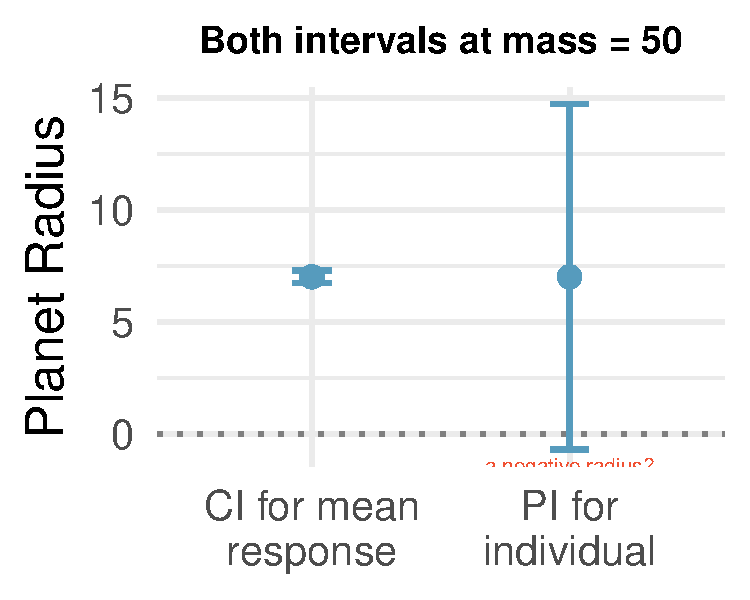
\includegraphics[width=0.95\textwidth]{ci_vs_pi_point.pdf}
\end{center}
}
{
{\small
\hl{CI for the mean:} $[6.73,\ 7.29]$, width $0.56$.

\vspace{0.7em}
\hl{PI for an individual:} $[-0.69,\ 14.71]$, width $15.39$, \textbf{$27\times$ wider}.

\vspace{0.7em}
Same $\hat y^\ast$. Same data. Same model. Different \emph{question}.}
}

\pause
\vspace{-0.2em}
\dq{The prediction interval's lower end is $-0.69$. What is wrong with that?}

\end{frame}


%%%%%%%%%%%%%%%%%%%%%%%%%%%%%%%%%%%%%%%%%%%%%%%%%%%%%%%%%%%%%%%%%%%%%%%%
\begin{frame}
\frametitle{Every $x$ has both, so both become bands}

\begin{center}
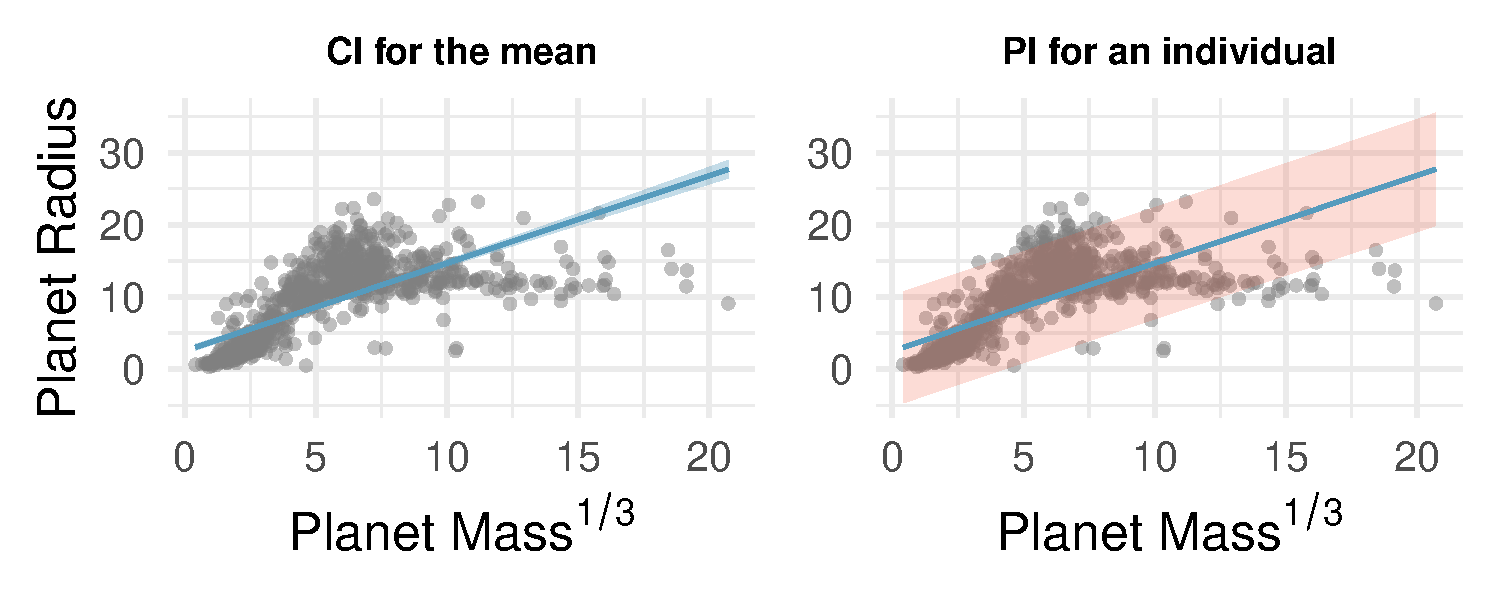
\includegraphics[width=0.90\textwidth]{ci_vs_pi_bands.pdf}
\end{center}

\pause
\vspace{-0.3em}
{\small The confidence band hugs the line: with $890$ planets we know where the \emph{line} is. The prediction band must contain the \emph{scatter}, and the scatter is what it is however much data we collect.}

\end{frame}


%%%%%%%%%%%%%%%%%%%%%%%%%%%%%%%%%%%%%%%%%%%%%%%%%%%%%%%%%%%%%%%%%%%%%%%%
\begin{frame}
\frametitle{The two standard errors}

\formula{The only difference is a $+1$}{With $s_e$ the residual standard deviation, at a new $x^\ast$: $$\mathrm{SE}_{\hat\mu} = s_e\sqrt{\tfrac{1}{n} + \tfrac{(x^\ast - \bar x)^2}{(n-1)s_x^2}}, \qquad \mathrm{SE}_{\hat y} = s_e\sqrt{\mathbf{1} + \tfrac{1}{n} + \tfrac{(x^\ast - \bar x)^2}{(n-1)s_x^2}}.$$}

\pause
\vspace{0.4em}
Both intervals are then the usual $\hat y^\ast \pm t^\ast_{\,n-2}\cdot\mathrm{SE}$, the same recipe as every interval since Lecture 13.

\pause
\vspace{0.2em}
{\small That lone $\mathbf{1}$ is the whole lecture. Where does it come from?}

\end{frame}


%%%%%%%%%%%%%%%%%%%%%%%%%%%%%%%%%%%%%%%%%%%%%%%%%%%%%%%%%%%%%%%%%%%%%%%%
\begin{frame}
\frametitle{Three terms, three sources of doubt}
$$\mathrm{SE}_{\hat y} = s_e\sqrt{\underbrace{1}_{\text{(1) the scatter}} + \underbrace{\tfrac{1}{n}}_{\text{(2) the line's height}} + \underbrace{\tfrac{(x^\ast - \bar x)^2}{(n-1)s_x^2}}_{\text{(3) the line's tilt}}}$$

\pause
\vspace{0.2em}
{\small
\begin{enumerate}
\item \textbf{The scatter.} Real planets do not sit \emph{on} the line. This is the term the CI does not have.
\item \textbf{The height.} We estimated $\hat\beta_0$ from data; the error shrinks like $1/n$.
\item \textbf{The tilt.} An error in $\hat\beta_1$ is harmless at $\bar x$ and grows as you move away.
\end{enumerate}}

\pause
\vspace{0.1em}
{\small On our planets, at $x^\ast$: $\;1$, $\;0.0011$, $\;0.0002$. \hl{The scatter is $99.9\%$ of it.}}

\end{frame}


%%%%%%%%%%%%%%%%%%%%%%%%%%%%%%%%%%%%%%%%%%%%%%%%%%%%%%%%%%%%%%%%%%%%%%%%
\begin{frame}
\frametitle{Term (3), drawn}

\twocol{0.52}{0.48}
{
\begin{center}
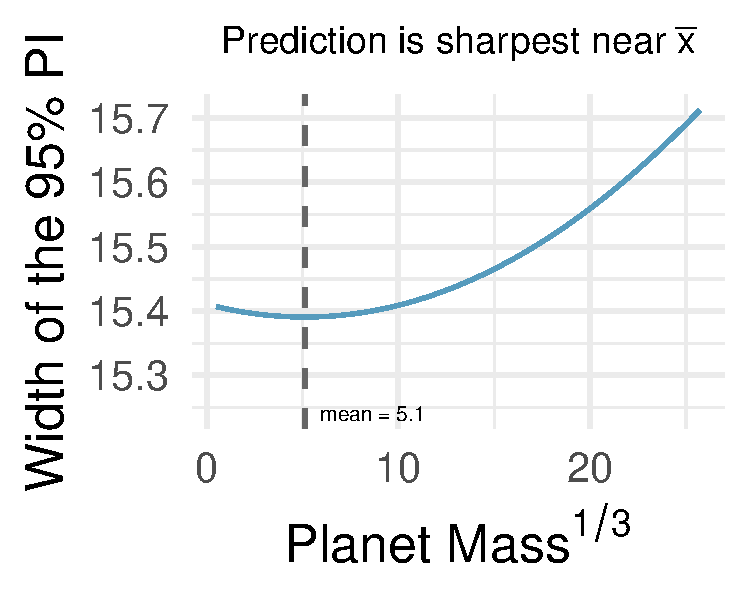
\includegraphics[width=0.95\textwidth]{band_width_xstar.pdf}
\end{center}
}
{
{\small The width of the prediction interval, as a function of \emph{where} you predict.

\vspace{0.7em}
A shallow parabola with its minimum at $\bar x$: prediction is sharpest in the middle of your data, blunter at the edges.

\vspace{0.7em}
\hl{But read the vertical scale.} It barely moves. Term (1) swamps the other two.}
}

\end{frame}


%%%%%%%%%%%%%%%%%%%%%%%%%%%%%%%%%%%%%%%%%%%%%%%%%%%%%%%%%%%%%%%%%%%%%%%%
\begin{frame}
\frametitle{What infinite data would, and would not, buy}

Let $n \to \infty$. Terms (2) and (3) both vanish:
$$\mathrm{SE}_{\hat\mu} \;\longrightarrow\; 0, \qquad\qquad \mathrm{SE}_{\hat y} \;\longrightarrow\; s_e .$$

\pause
\vspace{0.4em}
\keyidea{With enough data the \hl{confidence} interval shrinks to a point: we would know the mean radius at $x^\ast$ exactly. The \hl{prediction} interval never falls below $\pm t^\ast s_e$; on our data it stalls at a width of $15.4$ Earth radii. Individual planets vary, and no amount of data makes them stop.}

\end{frame}


%%%%%%%%%%%%%%%%%%%%%%%%%%%%%%%%%%%%%%%%%%%%%%%%%%%%%%%%%%%%%%%%%%%%%%%%
\section{Prediction after a transformation}
%%%%%%%%%%%%%%%%%%%%%%%%%%%%%%%%%%%%%%%%%%%%%%%%%%%%%%%%%%%%%%%%%%%%%%%%
\begin{frame}
\frametitle{That negative radius}

The prediction interval said a $50$-Earth-mass planet could have a radius of $-0.69$.

\pause
\vspace{0.4em}
\caution{The model is not confused. It is being faithful to what we told it to assume. We put \hl{normal errors on the raw radius scale}, and a normal distribution has no floor. Once $\hat y^\ast$ is close enough to zero relative to $s_e$, the interval walks straight through it.}

\pause
\vspace{0.4em}
Lecture 14 had already rejected this model on the \emph{diagnostics}: the residuals fanned out. Here is the same verdict in a form you cannot argue with: \hl{it predicts planets that cannot exist.}

\end{frame}


%%%%%%%%%%%%%%%%%%%%%%%%%%%%%%%%%%%%%%%%%%%%%%%%%%%%%%%%%%%%%%%%%%%%%%%%
\begin{frame}
\frametitle{Predicting with Lecture 14's model instead}

Fit $\log(\text{radius}) \sim \log(\text{mass})$, build the interval \emph{on the log scale}, exponentiate at the end. At $\text{mass} = 50$:

\pause
\vspace{0.3em}
{\footnotesize
\begin{center}
\setlength{\tabcolsep}{5pt}
\begin{tabular}{@{}lcccc@{}}
\toprule
& \textbf{interval} & \textbf{center} & \textbf{arms} & \\
\midrule
on the $\log$ scale & $[0.88,\ 2.57]$ & $1.72$ & $-0.84\ /\ +0.84$ & (symmetric) \\
back-transformed & $[2.42,\ 13.01]$ & $5.61$ & $-3.19\ /\ +7.40$ & \hl{(asymmetric)} \\
\bottomrule
\end{tabular}
\end{center}}

\pause
\vspace{0.3em}
{\small The upper arm is $2.3\times$ the lower, and the interval \hl{cannot cross zero}, since $e^{\text{anything}} > 0$. A symmetric interval in $\log y$ becomes a skewed one in $y$, exactly right for a quantity that is positive and right-skewed.}

\end{frame}


%%%%%%%%%%%%%%%%%%%%%%%%%%%%%%%%%%%%%%%%%%%%%%%%%%%%%%%%%%%%%%%%%%%%%%%%
\begin{frame}
\frametitle{The band, back on the planets' own scale}

\begin{center}
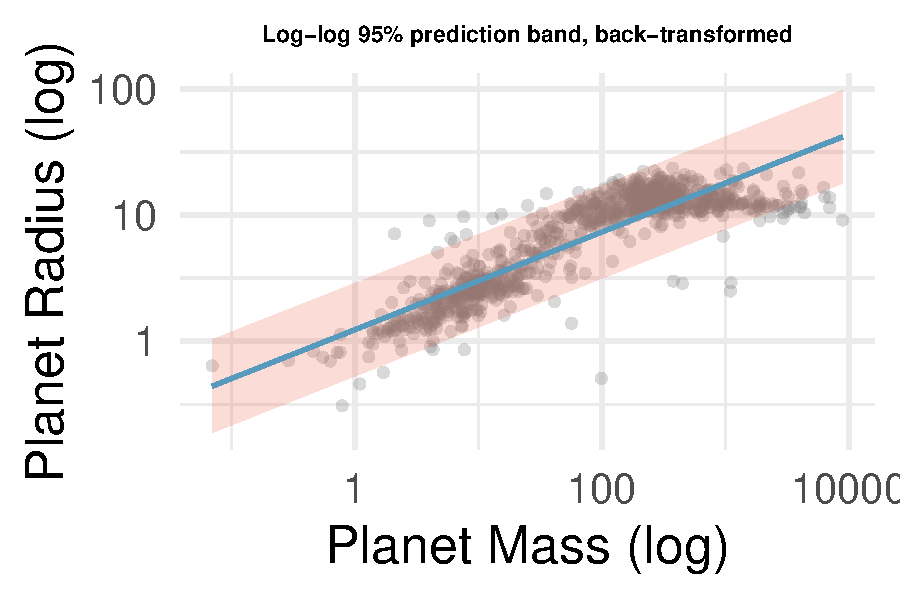
\includegraphics[width=0.55\textwidth]{loglog_prediction_band.pdf}
\end{center}

\pause
\vspace{-0.3em}
\keyidea{Transform, do \emph{all} the inference on the transformed scale, and back-transform \emph{last}. One catch: $e^{\hat\mu}$ is the predicted \hl{median}, not the mean.}

\end{frame}


%%%%%%%%%%%%%%%%%%%%%%%%%%%%%%%%%%%%%%%%%%%%%%%%%%%%%%%%%%%%%%%%%%%%%%%%
\section{Extrapolation}
%%%%%%%%%%%%%%%%%%%%%%%%%%%%%%%%%%%%%%%%%%%%%%%%%%%%%%%%%%%%%%%%%%%%%%%%
\begin{frame}
\frametitle{Predicting where you have no data}

Lecture 4 drew the line between \hl{interpolation} (inside the data) and \hl{extrapolation} (outside), and warned you off the second. Now we can watch what the \emph{intervals} do out there.

\pause
\vspace{0.2em}
\begin{center}
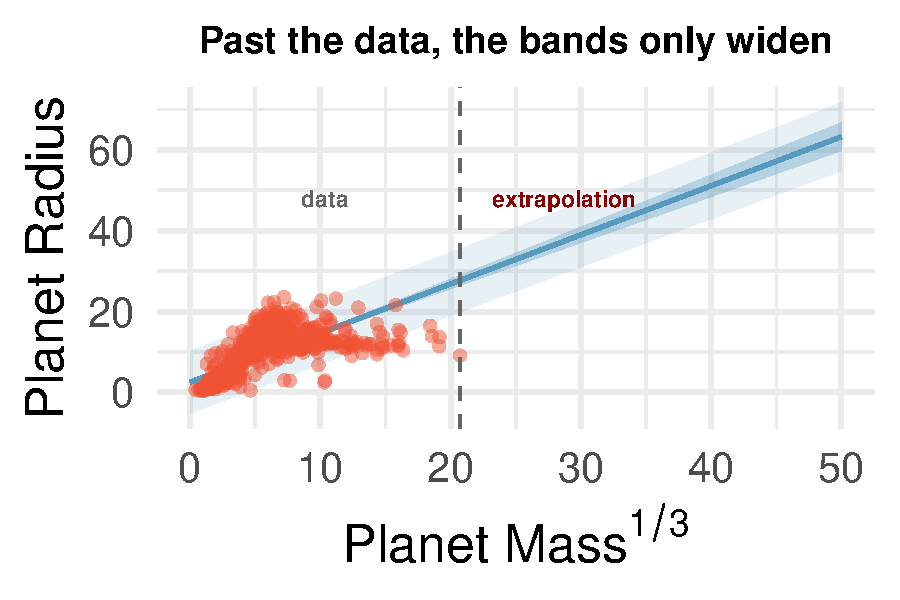
\includegraphics[width=0.58\textwidth]{extrapolation_bands.pdf}
\end{center}

\end{frame}


%%%%%%%%%%%%%%%%%%%%%%%%%%%%%%%%%%%%%%%%%%%%%%%%%%%%%%%%%%%%%%%%%%%%%%%%
\begin{frame}
\frametitle{The interval does not warn you}

{\small
\begin{center}
\begin{tabular}{@{}lrr@{}}
\toprule
predicting at $\text{mass}^{1/3} =$ & $\hat y^\ast$ & PI width \\
\midrule
$5.1$ \quad (the center of the data) & $8.7$ & $15.39$ \\
$20.7$ \quad (the last planet we have) & $27.7$ & $15.58$ \\
$50.0$ \quad (far outside anything observed) & $63.2$ & $16.86$ \\
\bottomrule
\end{tabular}
\end{center}}

\pause
\vspace{0.2em}
The band widens by \emph{ten percent} over that entire journey. It looks perfectly healthy.

\pause
\vspace{0.2em}
\caution{But $63.2$ Earth radii is larger than any planet known, since Jupiter is $11$. The model is confidently, precisely wrong. \hl{Extrapolation is dangerous not because the interval blows up, but because it does not.} Nothing in the arithmetic knows the data ran out.}

\end{frame}


%%%%%%%%%%%%%%%%%%%%%%%%%%%%%%%%%%%%%%%%%%%%%%%%%%%%%%%%%%%%%%%%%%%%%%%%
\section{Polynomial models}
%%%%%%%%%%%%%%%%%%%%%%%%%%%%%%%%%%%%%%%%%%%%%%%%%%%%%%%%%%%%%%%%%%%%%%%%
\begin{frame}
\frametitle{When a straight line is not enough}

Lecture 14 bent the model by \emph{transforming} a variable. The other way is to add \hl{powers} of it:
$$y = \beta_0 + \beta_1 x + \beta_2 x^2 + \varepsilon, \qquad y = \beta_0 + \beta_1 x + \beta_2 x^2 + \beta_3 x^3 + \varepsilon, \ \ldots$$

\pause
\vspace{0.3em}
\keyidea{A polynomial regression is still a \hl{linear model}, linear \emph{in the parameters} $\beta_j$, which is all least squares ever asked for. So \texttt{lm()}, the $t$ tests, the intervals and the LINE checks all carry over unchanged. ``Non-linear'' describes the \emph{curve}, not the algebra.}

\pause
\vspace{0.2em}
{\small In R: \texttt{lm(y \textasciitilde{} poly(x, 3))}. Each extra degree buys one more bend.}

\end{frame}


%%%%%%%%%%%%%%%%%%%%%%%%%%%%%%%%%%%%%%%%%%%%%%%%%%%%%%%%%%%%%%%%%%%%%%%%
\begin{frame}
\frametitle{And when a polynomial extrapolates}

\begin{center}
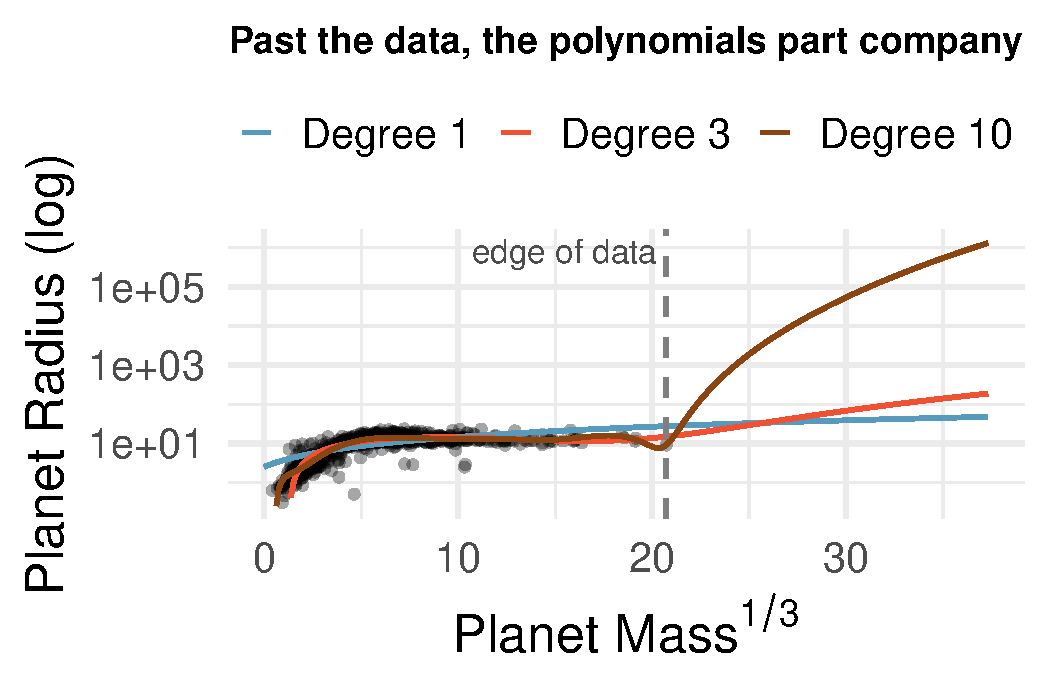
\includegraphics[width=0.64\textwidth]{polynomial_extrapolation.pdf}
\end{center}

\pause
\vspace{-0.3em}
{\small At $1.5\times$ the edge of the data the three models predict a radius of $40$, $81$, and \hl{$93{,}511$} Earth radii. The degree-$10$ curve was the \emph{best} fit inside the data ($R^2 = 0.82$). Outside it, a high-degree polynomial is not a model. It is a catapult.}

\end{frame}


%%%%%%%%%%%%%%%%%%%%%%%%%%%%%%%%%%%%%%%%%%%%%%%%%%%%%%%%%%%%%%%%%%%%%%%%
\section{Overfitting}
%%%%%%%%%%%%%%%%%%%%%%%%%%%%%%%%%%%%%%%%%%%%%%%%%%%%%%%%%%%%%%%%%%%%%%%%
\begin{frame}
\frametitle{Fits better, predicts worse}

Take a realistic sample of $n = 60$ planets, not all $890$, and raise the degree.

\pause
\vspace{0.1em}
\begin{center}
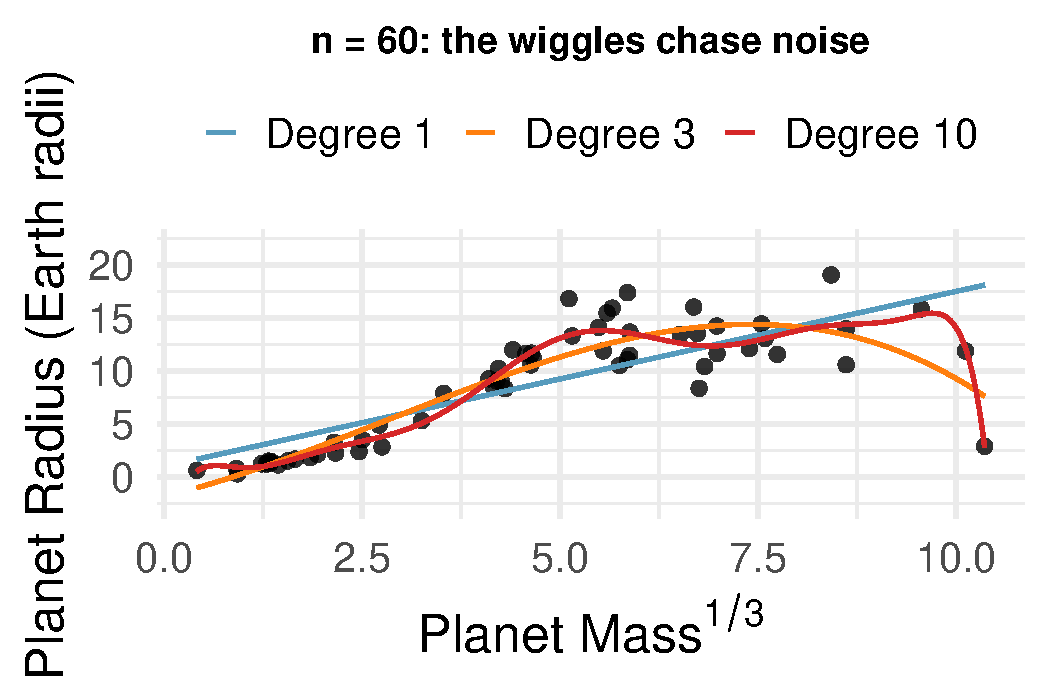
\includegraphics[width=0.60\textwidth]{overfit_demo.pdf}
\end{center}

\pause
\vspace{-0.4em}
{\small The degree-$10$ curve threads through the points beautifully. It is chasing \hl{noise}, and noise does not repeat in the next sample.}

\end{frame}


%%%%%%%%%%%%%%%%%%%%%%%%%%%%%%%%%%%%%%%%%%%%%%%%%%%%%%%%%%%%%%%%%%%%%%%%
\begin{frame}
\frametitle{You cannot grade a model on the data that trained it}

\keyidea{In-sample $R^2$ can only ever \emph{rise} as you add terms: a degree-$10$ polynomial will always ``explain'' more of the training data than a line does. Judging a model by how well it fits the data it was fitted to is grading your own homework.}

\pause
\vspace{0.4em}
Lecture 7 gave us two tools that try to correct for exactly this: \hl{adjusted $R^2$} and \hl{AIC}. Both subtract a penalty for the number of parameters.

\pause
\vspace{0.4em}
\dq{Are they enough? Each was derived under assumptions, so what happens when we push them to degree $10$ on $60$ points?}

\end{frame}


%%%%%%%%%%%%%%%%%%%%%%%%%%%%%%%%%%%%%%%%%%%%%%%%%%%%%%%%%%%%%%%%%%%%%%%%
\section{Cross-validation}
%%%%%%%%%%%%%%%%%%%%%%%%%%%%%%%%%%%%%%%%%%%%%%%%%%%%%%%%%%%%%%%%%%%%%%%%
\begin{frame}
\frametitle{Where the two penalties come from, and stop}

\begin{itemize}
\item \textbf{Adjusted $R^2$} penalises parameters, but its penalty is derived \hl{specifically for linear regression, assuming the model is correct}. Outside that, it has nothing to say.
\pause
\item \textbf{AIC} is more general (it needs only a likelihood) but its $+2k$ penalty is an \hl{asymptotic} approximation, trustworthy when $n$ is far larger than $k$. At $n = 60$ with $k = 11$, that is a stretch.
\end{itemize}

\pause
\vspace{0.5em}
Both are \emph{theories} about how badly a model will generalize.

\pause
\vspace{0.3em}
\hl{So why theorize?} We could hide some data, fit without it, and \emph{look}.

\end{frame}


%%%%%%%%%%%%%%%%%%%%%%%%%%%%%%%%%%%%%%%%%%%%%%%%%%%%%%%%%%%%%%%%%%%%%%%%
\begin{frame}
\frametitle{$k$-fold cross-validation}

\formula{The algorithm}{%
\begin{enumerate}\setlength{\itemsep}{1pt}
\item Choose an error measure: squared error $(y_i - \hat y_i)^2$, absolute error, or a negative log-likelihood.
\item Split the data into $k$ equal \hl{folds}.
\item For each fold $j$: fit on the \emph{other} $k-1$ folds, predict fold $j$, record its average error $\mathrm{err}_j$.
\end{enumerate}
$$\text{CV-error} \;=\; \frac{1}{k}\sum_{j=1}^{k} \mathrm{err}_j .$$}

\pause
\vspace{0.3em}
{\small Every observation gets predicted exactly once, by a model that \hl{never saw it}. Lower CV-error means better prediction on data you do not have. Usually $k = 5$ or $10$.}

\end{frame}


%%%%%%%%%%%%%%%%%%%%%%%%%%%%%%%%%%%%%%%%%%%%%%%%%%%%%%%%%%%%%%%%%%%%%%%%
\begin{frame}
\frametitle{One split is not enough}

\caution{At $n = 60$ a single $5$-fold split gives a \emph{jumpy} answer: the winning degree moves around depending on where the folds happened to fall. So repeat the whole procedure with fresh splits (here, $20$ times) and average. Every curve that follows is a repeated-CV curve.}

\pause
\vspace{0.4em}
{\small This is not a technicality. Cross-validation \emph{estimates} a quantity, and like any estimate it has a standard error. One split is a sample of size one.}

\end{frame}


%%%%%%%%%%%%%%%%%%%%%%%%%%%%%%%%%%%%%%%%%%%%%%%%%%%%%%%%%%%%%%%%%%%%%%%%
\begin{frame}
\frametitle{Adjusted $R^2$ chooses degree 10}

\begin{center}
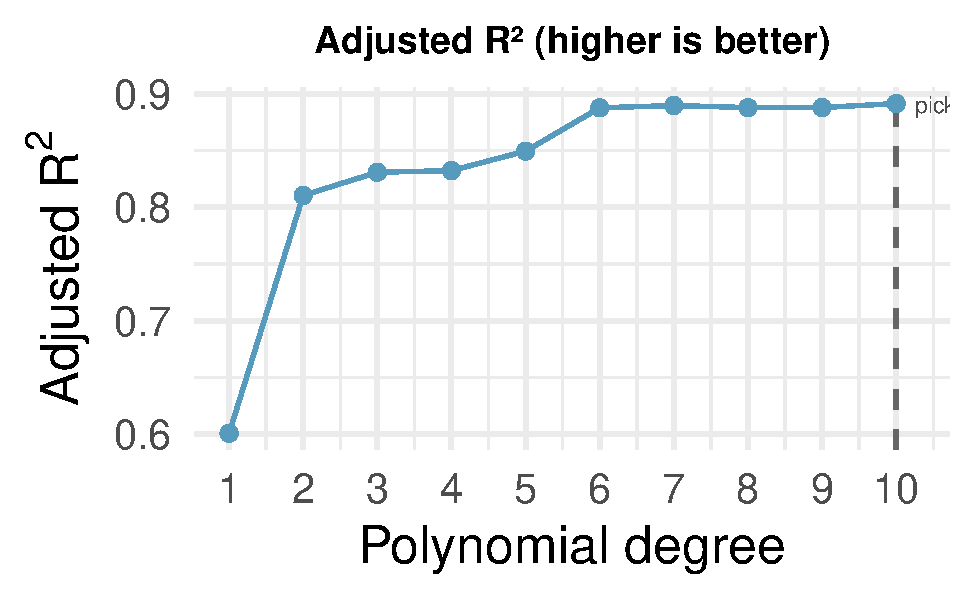
\includegraphics[width=0.58\textwidth]{adjr2_by_degree.pdf}
\end{center}

\pause
\vspace{-0.3em}
{\small It rises, essentially without pause, all the way to the most complex model on offer. The penalty is real, but far too gentle to hold back a degree-$10$ polynomial fitted to $60$ points.}

\end{frame}


%%%%%%%%%%%%%%%%%%%%%%%%%%%%%%%%%%%%%%%%%%%%%%%%%%%%%%%%%%%%%%%%%%%%%%%%
\begin{frame}
\frametitle{AIC does better, and still cannot see the cliff}

\begin{center}
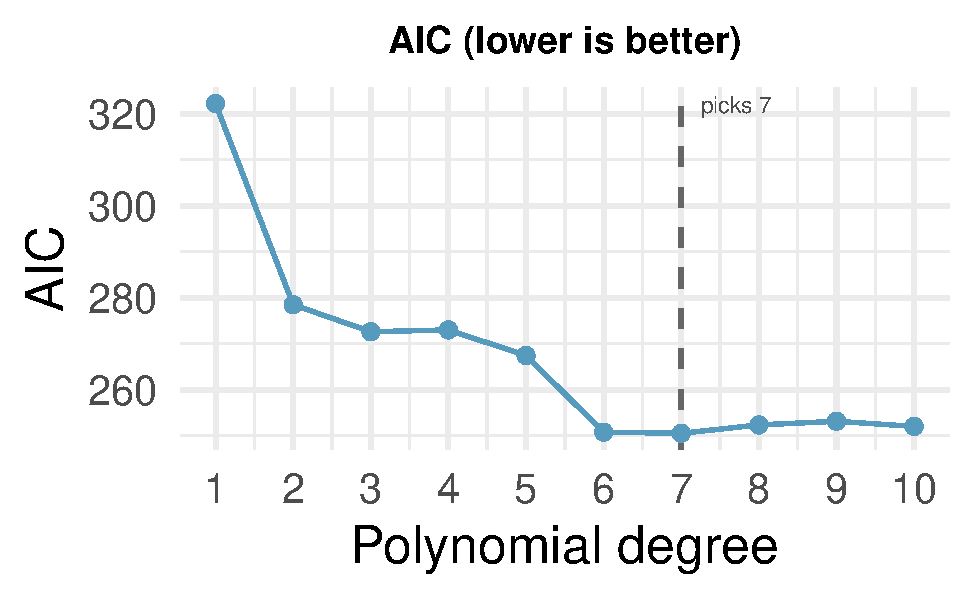
\includegraphics[width=0.58\textwidth]{aic_by_degree.pdf}
\end{center}

\pause
\vspace{-0.3em}
{\small AIC stops at degree $7$, a real improvement. But its curve is nearly \emph{flat} from $6$ to $10$: it sees nothing alarming about the highest degrees.}

\end{frame}


%%%%%%%%%%%%%%%%%%%%%%%%%%%%%%%%%%%%%%%%%%%%%%%%%%%%%%%%%%%%%%%%%%%%%%%%
\begin{frame}
\frametitle{Cross-validation sees the cliff}

\begin{center}
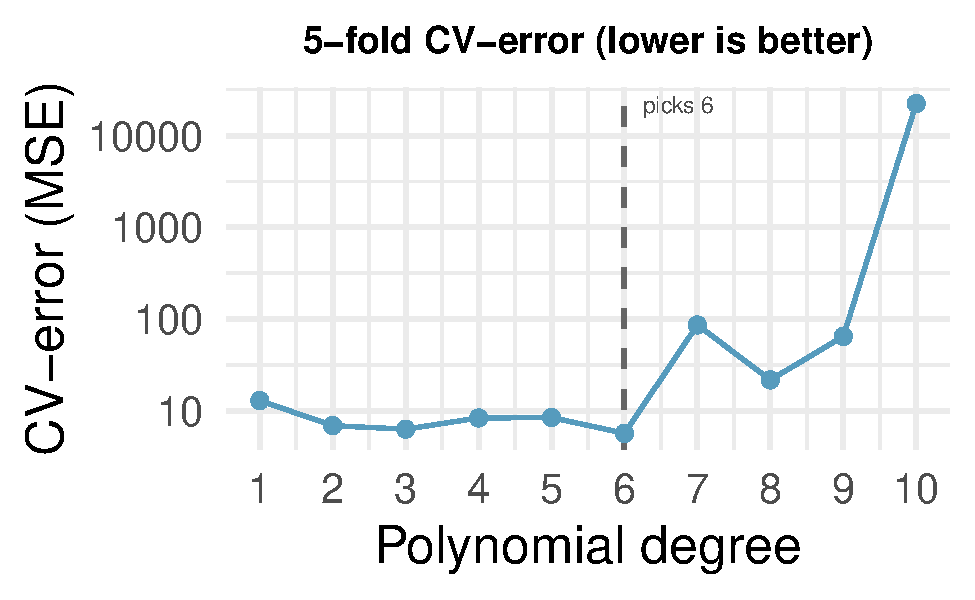
\includegraphics[width=0.58\textwidth]{cv_comparison.pdf}
\end{center}

\pause
\vspace{-0.3em}
{\small \emph{(Log scale, or it would not fit.)} The error falls, flattens, then \hl{explodes}: at degree $10$ it is roughly $4{,}000\times$ its minimum. Meanwhile adjusted $R^2$ was still going \emph{up}.}

\end{frame}


%%%%%%%%%%%%%%%%%%%%%%%%%%%%%%%%%%%%%%%%%%%%%%%%%%%%%%%%%%%%%%%%%%%%%%%%
\begin{frame}
\frametitle{The same ten models, four verdicts}

{\small
\begin{center}
\setlength{\tabcolsep}{4pt}
\begin{tabular}{@{}lcl@{}}
\toprule
\textbf{Criterion} & \textbf{Picks} & \textbf{What it is really doing} \\
\midrule
$R^2$ & $10$ & rewards complexity, always. \hl{Never use it.} \\
Adjusted $R^2$ & $10$ & a penalty, but built for a \emph{correct} linear model \\
AIC & $7$ & a likelihood penalty: asymptotic, wants $n \gg k$ \\
\hl{CV-error} & $6$ & \hl{measures prediction on data it never saw} \\
\bottomrule
\end{tabular}
\end{center}}

\pause
\vspace{0.2em}
\keyidea{The point is not which degree wins; $6$ and $7$ are a coin toss here. It is that only cross-validation \hl{punishes} the catastrophic models, with no assumption that the model is correct, no asymptotics, and for \emph{any} model you can fit and predict from.}

\end{frame}


%%%%%%%%%%%%%%%%%%%%%%%%%%%%%%%%%%%%%%%%%%%%%%%%%%%%%%%%%%%%%%%%%%%%%%%%
\section{Wrap-up}
%%%%%%%%%%%%%%%%%%%%%%%%%%%%%%%%%%%%%%%%%%%%%%%%%%%%%%%%%%%%%%%%%%%%%%%%
\begin{frame}
\frametitle{Summary: the two intervals}

\begin{itemize}
\item One fitted value, \hl{two questions}: the \emph{mean} response at $x^\ast$ (a confidence interval), or \emph{one new} observation (a prediction interval).
\item The prediction interval carries an extra $s_e^2$, the irreducible scatter. It shrinks to $\pm t^\ast s_e$, never to zero. On our planets it is \hl{$27\times$} the CI.
\item Its three terms: the \hl{scatter} (which dominates), the line's \hl{height}, the line's \hl{tilt} (worst far from $\bar x$).
\item Transform, infer on the transformed scale, back-transform \emph{last}: a symmetric log interval becomes an \hl{asymmetric, strictly positive} one.
\item \hl{Extrapolation} is dangerous because the interval stays narrow while the model goes wrong.
\end{itemize}

\end{frame}


%%%%%%%%%%%%%%%%%%%%%%%%%%%%%%%%%%%%%%%%%%%%%%%%%%%%%%%%%%%%%%%%%%%%%%%%
\begin{frame}
\frametitle{Summary: choosing a model}

\begin{itemize}
\item A \hl{polynomial} is still a linear model, linear in the parameters, so all the usual inference tools apply. But it \emph{overfits}: in-sample $R^2$ can only rise with degree.
\item So a model cannot be graded on the data that trained it. \hl{Adjusted $R^2$} and \hl{AIC} try, but each rests on assumptions that fail for a flexible model on a small sample.
\item \hl{Cross-validation} grades a model on data it has never seen. It assumes only independence, and it is the one criterion that punishes the models that predict catastrophically.
\item Repeat the folds and average: a single split is a sample of size one.
\end{itemize}

\end{frame}


%%%%%%%%%%%%%%%%%%%%%%%%%%%%%%%%%%%%%%%%%%%%%%%%%%%%%%%%%%%%%%%%%%%%%%%%
\begin{frame}
\frametitle{Coming up next}

\hl{Lecture 16: logistic regression inference.} Module 3's last act, and everything today generalizes to it.

\vspace{0.4em}
\begin{itemize}
\item The response goes \hl{binary}: survived / did not. Coefficients become \hl{odds ratios}, and their confidence intervals with them.
\item Squared error is meaningless for a $0/1$ outcome, so the \emph{loss} changes: the \hl{Brier score}, the \hl{log-loss}. Then the \emph{same} $k$-fold machinery runs on top of it, unchanged.
\end{itemize}

\vspace{0.4em}
{\small Cross-validation is not a regression trick. It is how you grade any model at all. IMS Ch.\ 26.}

\end{frame}


%%%%%%%%%%%%%%%%%%%%%%%%%%%%%%%%%%%%%%%%%%%%%%%%%%%%%%%%%%%%%%%%%%%%%%%%
% Activity
%%%%%%%%%%%%%%%%%%%%%%%%%%%%%%%%%%%%%%%%%%%%%%%%%%%%%%%%%%%%%%%%%%%%%%%%
\begin{frame}
\frametitle{Activity: what is this house worth?}

\activity{$2{,}930$ houses sold in Ames, Iowa. Predict a sale price from living area and whatever else earns its place: but decide \emph{first} which of the two intervals the question calls for. Then choose a polynomial degree by cross-validation, and see whether adjusted $R^2$ agrees with you.}

\vspace{0.3em}
{\small
\begin{itemize}
\item Work in \emph{pairs} (analyst + guide); one worksheet per pair.
\item We pause for check-ins. \hl{Be ready to share}.
\item Data and starter code are on Blackboard; reference these slides as you go.
\end{itemize}}

\end{frame}


%%%%%%%%%%%%%%%%%%%%%%%%%%%%%%%%%%%%%%%%%%%%%%%%%%%%%%%%%%%%%%%%%%%%%%%%
\begin{frame}
\frametitle{Compare with the groups around you}

\textbf{When you reach the end of Part 5:}

\vspace{0.3em}
\begin{enumerate}
\item Compare your final model with at least two neighboring pairs.
\item Did cross-validation choose the same degree for everyone? If not, why not?
\item Whose interval would you actually quote to someone selling a house, and is it a CI or a PI?
\item Having heard them, would you change your model? Say why, or why not.
\end{enumerate}

\vspace{0.5em}
\hl{Write your answers in the box at the end of the worksheet.}

\end{frame}


%%%%%%%%%%%%%%%%%%%%%%%%%%%%%%%%%%%%%%%%%%%%%%%%%%%%%%%%%%%%%%%%%%%%%%%%
% End document
%%%%%%%%%%%%%%%%%%%%%%%%%%%%%%%%%%%%%%%%%%%%%%%%%%%%%%%%%%%%%%%%%%%%%%%%

\end{document}
